\chapter{CH PLIF Signal Modeling and Validation}
\label{ch:chplif}

% This chapter covers the modeling of the CH PLIF signal and contains the following sections:

% 0. Preliminary experiments
%   0.1 Excitation scan
%   0.2 Linearity test
% 1. Signal modeling
%     1.1 Constants, assumptions, simplifications
%     1.2 Comparison of models (GRI, USCv2, Syngas, C1-C3, San Diego, etc.) / CH₄+air results
% 2. Results
%   Unstrained, laminar flames
%     2.1 Methane + air flames
%         2.1.1 subsection comparison with experiments
%     2.2 C1-C3 alkanes flames
%     2.3 Syngas mixtures
%     2.4 Syngas + C1-C3 alkanes
%   Strained laminar flames
%     2.5 Strain effects

% Questions to be answered (from proposal):

% 1. Detailing the development of a CH PLIF system (covered in Chapter 2,3 and here)
% 2. Demonstration on an atmospheric pressure laminar flame
% 3. Validate with quenching models
% 4. Model signal for strained flames
% 5. Model signal for fuel mixtures

% TODO:Write a short introduction to the chapter to start it off

\section{CH PLIF Preliminary Experiments}
\label{sec:chplif-preliminary-experiments}

The CH PLIF imaging system was evaluated for use in imaging hydrocarbon flames by performing two preliminary experiments.
First, an excitation scan was performed to confirm the location of the optimal wavelength to excite the CH radicals in a typical hydrocarbon flame.
Second, a test of the linearity of the LIF signal with respect to the incident laser intensity was performed.
The setup and results of these experiments are described in the following subsections.

\subsection{Excitation Scan}
\label{subsec:prelim-excitation-scan}

\begin{figure}

\centering

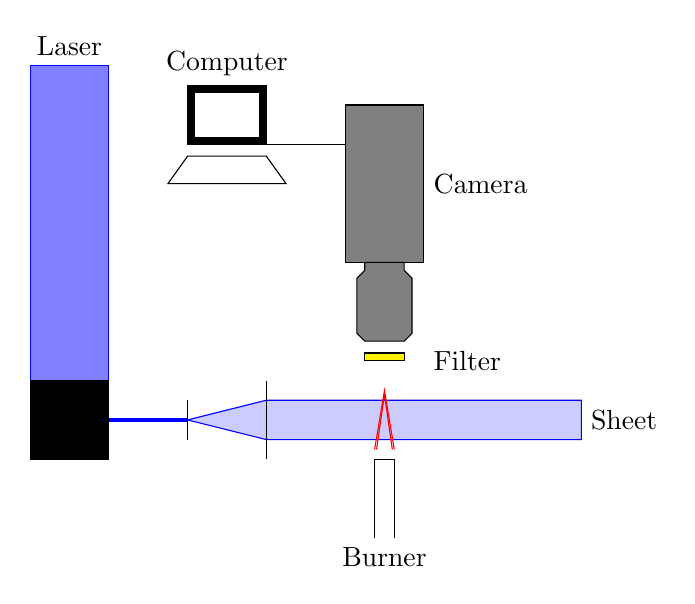
\begin{tikzpicture}

% Laser
\filldraw [fill=blue!50!white, draw=blue] ( 0, 5 ) rectangle ++( 1, -4 );
\filldraw [black] ( 0, 1 ) rectangle ++( 1, -1 );

% Beam
\draw [very thick, blue] ( 1, 0.5 ) -- ++( 1, 0 );
\draw [draw=blue,fill=blue!20!white] ( 2, 0.5 ) -- ++( 1, 0.25 ) -- ++( 4, 0 ) -- ++( 0, -0.5 ) -- ++( -4, 0 ) -- cycle;

% Lenses
\draw ( 2, 0.25 ) -- ++( 0, 0.5 );
\draw ( 3, 0 ) -- ++( 0, 1 );

% Laminar burner
\draw ( 4.375, -1 ) -- ++( 0, 1 ) -- ++( 0.25, 0 ) -- ++( 0, -1 );

% Flame
\draw [red] ( 4.375, 0.125 ) -- ++( 0.125, 0.75 ) -- ++( 0.125, -0.75 );
\draw [red] ( 4.4, 0.125 ) -- ++( 0.1, 0.7 ) -- ++( 0.1, -0.7 );

% Camera
\filldraw [fill=black!50!white, draw=black] ( 4, 4.5 ) rectangle ++( 1, -2 );
\filldraw [fill=black!50!white, draw=black] ( 4.25, 2.5 ) -- ++( 0, -0.1 ) -- ++( -0.1, -0.1 ) -- ++( 0, -0.7 ) -- ++( 0.1, -0.1 ) -- ++( 0.5, 0 ) -- ++( 0.1, 0.1 ) -- ++( 0, 0.7 ) -- ++( -0.1, 0.1 ) -- ++ ( 0, 0.1 ) -- cycle;

% Filter
\filldraw [fill=yellow, draw=black] ( 4.25, 1.25 ) rectangle ++( 0.5, 0.1 );

% Computer
\filldraw [black] ( 2, 4 ) rectangle ++( 1, 0.75 );
\filldraw [white]( 2.1, 4.1 ) rectangle ++( 0.8, 0.55 );
\draw ( 2, 3.85 ) -- ++( 1, 0 ) -- ++( 0.25, -0.35 ) -- ++( -1.5, 0 ) -- cycle;

\draw ( 3, 4 ) -- ++( 1, 0 );

% Labels
\node at ( 0.5, 5 ) [above] {Laser};
\node at ( 2.5, 4.75 ) [above] {Computer};
\node at ( 5, 3.5 ) [right] {Camera};
\node at ( 5, 1.25 ) [right] {Filter};
\node at ( 4.5, -1 ) [below] {Burner};
\node at ( 7, 0.5 ) [right] {Sheet};

\end{tikzpicture}

\caption[Schematic of the excitation scan experiment]{The figure above shows the schematic of the excitation scan experiment. Optics form the laser beam into a collimated sheet focused over a laminar Bunsen burner. The fluorescence is imaged perpendicularly by an intensified camera synchronized to the laser pulse. A 3 mm GG 420 filter is used to reject elastic scattering.}

\label{fig:excitationScan}

\end{figure}


\begin{figure}

\centering

\input{figures/excitationScanFlameImage}

\caption[Excitation scan processing]{FIXME.}

\label{fig:excitationScanFlame}

\end{figure}


\begin{figure}

\centering

\input{figures/excitationScanResultsPlot}

\caption[Results of the excitation scan experiment]{The plot above shows the mean signal level of an emitting pixel determined by three separate analysis methods. They are compared to a simulated excitation scan from LIFBASE.}

\label{fig:excitationScanResults}

\end{figure}



An excitation scan is performed by tuning the output of the alexandrite laser from \(\lambda\) = 387.077 nm to 387.260 nm.
This serves two purposes.
First, it locates the optimal wavelength to excite the CH radicals that results in the highest fluorescence yield.
Second, the variation of the signal intensity can be compared with simulated profiles from LIFBASE or other spectroscopic calculations and our estimation of the laser linewidth can be validated.
The laser linewidth is an integral parameter and appears in the absorption integral used by the models developed in Chapter \ref{ch:background}.

A schematic of the excitation scan experiment is shown in Figure \ref{fig:excitationScan}.
The intensified PI Acton 512\(\times\)512 camera described in Section \ref{subsec:experimental-ch-chemiluminescence} is used to image a premixed, laminar methane-air flame operating at close to stoichiometric conditions.
The laminar flame is stabilized on the Bunsen burner described in Section \ref{subsubsec:plif-laminar-flame-setup}.
The alexandrite laser is operated at a power of 16 mJ/pulse in the second harmonic.
The sheet forming optics consist of a +50 mm cylindrical lens and a +250 mm spherical lens placed 300 mm apart.
The optics form the beam into a collimated sheet about 25 mm (1 in) tall, focused to a thickness on the order of 250 \(\mu\)m at the flame location.
The sheet passes through the center of the flame and the edges of the sheet are blocked by razor blades to prevent reflections from the burner from saturating the camera.

The induced fluorescence in the flame sheet is imaged perpendicularly by the intensified camera using an 85 mm f/1.8 Nikon AF Nikkor lens.
A 3 mm thick 50 mm\(\times\)50 mm square GG 420 Schott glass filter is used to reject elastic scattering at the excitation wavelength.
This setup gives a magnification of approximately 62 \(\mu\)m/pixel.
The camera is triggered by the flash lamp sync signal from the laser system and the intensifier is gated over 300 ns, encompassing the 70 ns laser pulse.
The long gate width gives the intensifier enough time to prepare to receive the fluorescence, preventing signal loss due to irising.
The gate width is still short enough that minimal flame chemiluminescence or ambient lighting is recorded in the images.
100 instantaneous images are acquired for each excitation wavelength to acquire a good estimate of the mean fluorescence signal, \(\mu_{sig}\).

Figure \ref{fig:excitationScanFlame} shows a sample CH PLIF image from this dataset.
The images are background-corrected by subtracting the laser scattering (recorded without the flame).
The fluorescence signal is calculated from these images using three alternate approaches.

In Method I, two windows are identified that include the straight sections of the laminar flame.
The average fluorescence signal in each frame is calculated by taking the average of all the emitting pixels in the two windows.
A pixel is designated as an emitting pixel if its intensity exceeds the standard deviation of a typical background pixel by at least a factor of five.
The average of this value over all the frames is designated as the mean fluorescence signal, \(\mu_{sig}\).
In Method II, the intensity of the pixels is integrated over a straight line connecting the inner and outer edges of the flame.
The straight line is chosen along the beam so that the beam intensity does not vary along the integration path.
The integration is performed on the left and right arms of the flame, giving two readings per frame.
The mean of these values over all the frames is recorded as the mean fluorescence signal, \(\mu_{sig}\).
In Method III, the midpoints of the flame along the straight lines from Method II are located and the average of their intensities, over all the frames is recorded as the mean fluorescence signal, \(\mu_{sig}\).
The regions of interest for each of these methods are highlighted in Figure \ref{fig:excitationScanFlame}.

The result of this investigation is shown in Figure \ref{fig:excitationScanResults}.
The calculated mean fluorescence signals from the three methods are plotted against a LIFBASE simulation of the absorption spectrum of the CH \(B-X\) transition.
The profiles are appropriately scaled to match the LIFBASE simulation at the maximum value and at the minimum value.
The LIFBASE simulation is performed for a thermalized system at 1800 K, at atmospheric pressure.
Further, the instrument linewidth is specified to be the same as our estimate of the laser linewidth (1.06 \AA).

The line and midpoint methods use fewer pixels to calculate the mean and show minor deviations from the predicted results.
The window method uses more pixels and shows much smoother agreement with the simulated profile.
In general, the agreement between the measurements and the calculations is excellent.
The agreement is in fact so good that a minor adjustment to the calibration of the laser wavelength could be made using these results.

The results indicate that the optimal excitation wavelength, corresponding to the highest mean fluorescence signal, is about 387.2 nm.
For the rest of the experiments performed in this work, the laser is operated at this wavelength.
The results also help fine tune the calibration of the micrometer over this small region of the spectrum.
Finally, the results validate that our estimated laser linewith, 1.06 \AA, is accurate.
This value can now be used in subsequent calculations of the LIF signal levels.

\subsection{Linearity Test}
\label{subsec:prelim-linearity-test}

\begin{figure}

\centering

\begin{tikzpicture}

% Laser
\filldraw [fill=blue!50!white, draw=blue] ( 0, 5 ) rectangle ++( 1, -4 );
\filldraw [black] ( 0, 1 ) rectangle ++( 1, -1 );

% Beam
\draw [very thick, blue] ( 1, 0.5 ) -- ++( 9, 0 );

% Laminar burner
\draw ( 8.375, -1 ) -- ++( 0, 1 ) -- ++( 0.25, 0 ) -- ++( 0, -1 );

% Flame
\draw [red] ( 8.375, 0.125 ) -- ++( 0.125, 0.75 ) -- ++( 0.125, -0.75 );
\draw [red] ( 8.4, 0.125 ) -- ++( 0.1, 0.7 ) -- ++( 0.1, -0.7 );

% Screen
\draw [pattern = north east lines] ( 6.5, 0.6 ) rectangle ++( 0.1, 2.5 );
\draw [pattern = north east lines] ( 6.5, 0.4 ) rectangle ++( 0.1, -1 );

% Attenuators
\draw [fill = blue!35!white, draw = black] ( 2, 0.75 ) -- ++( 0.4, 1 ) -- ++( 0.1, 0 ) -- ++( -0.4, -1 ) --cycle;
\draw [fill = blue!35!white, draw = black] ( 2.25, 0.75 ) -- ++( 0.4, 1 ) -- ++( 0.1, 0 ) -- ++( -0.4, -1 ) --cycle;
\draw [fill = blue!35!white, draw = black] ( 2.5, 0.25 ) -- ++( 0.4, 1 ) -- ++( 0.1, 0 ) -- ++( -0.4, -1 ) --cycle;
\draw [fill = blue!35!white, draw = black] ( 3, 0.75 ) -- ++( 0.4, 1 ) -- ++( 0.1, 0 ) -- ++( -0.4, -1 ) --cycle;

% Camera
\filldraw [fill=black!50!white, draw=black] ( 8, 4.5 ) rectangle ++( 1, -2 );
\filldraw [fill=black!50!white, draw=black] ( 8.25, 2.5 ) -- ++( 0, -0.1 ) -- ++( -0.1, -0.1 ) -- ++( 0, -0.7 ) -- ++( 0.1, -0.1 ) -- ++( 0.5, 0 ) -- ++( 0.1, 0.1 ) -- ++( 0, 0.7 ) -- ++( -0.1, 0.1 ) -- ++ ( 0, 0.1 ) -- cycle;

% Filter
\filldraw [fill=yellow, draw=black] ( 8.25, 1.25 ) rectangle ++( 0.5, 0.1 );

% Computer
\filldraw [black] ( 6, 4 ) rectangle ++( 1, 0.75 );
\filldraw [white]( 6.1, 4.1 ) rectangle ++( 0.8, 0.55 );
\draw ( 6, 3.85 ) -- ++( 1, 0 ) -- ++( 0.25, -0.35 ) -- ++( -1.5, 0 ) -- cycle;

\draw ( 7, 4 ) -- ++( 1, 0 );

% Labels
\node at ( 0.5, 5 ) [above] {Laser};
\node at ( 3, 2 ) [above] {Attenuators};
\node at ( 6.5, -0.75 ) [below] {Screen};
\node at ( 6.5, 4.75 ) [above] {Computer};
\node at ( 9, 3.5 ) [right] {Camera};
\node at ( 9, 1.25 ) [right] {Filter};
\node at ( 8.5, -1 ) [below] {Burner};

\end{tikzpicture}

\caption[Schematic of the linearity experiment]{A schematic of the experimental setup used to perform the linearity experiment is shown. An unrefracted beam from the laser is directed at a laminar flame and imaged perpendicularly. The beam energy is progressively attenuated by introducing multiple quartz blocks and disks. The drift in the beam is minimized by using attenuating elements in pairs so that any beam deviation is compensated.}

\label{fig:linearityTest}

\end{figure}


\begin{figure}

\centering

\input{figures/linearityResultsPlot}

\caption[Results of the linearity experiment]{The plot above shows the results of the linearity experiment. The LIF signal intensity is measured for a range of input laser energies (expressed here an an intensity). The data points below 1 J/cm\(^2\) are marked in \textcolor{blue}{blue} and fitted to a linear curve. One outlier (\textcolor{red}{red}), along with data points at high laser intensities are not included in the linear fit.}

\label{fig:linearityResults}

\end{figure}



As explained in Chapter \ref{ch:background}, the variation of the fluorescence signal with the excitation laser intensity exhibits a saturation curve.
For reasons mentioned in that discussion, we prefer to operate in the weak excitation limit where the fluorescence signal scales linearly with the input laser energy.
Further, the models developed in Section \ref{sec:background-chplif-signal-modeling} use fluorescence yield expressions that are only valid in the linear regime.
Hence, an experiment is performed to verify the linearity of the system response at the intensities at which the flames are imaged for this work.

The schematic of the setup is shown in Figure \ref{fig:linearityTest}.
The laser is tuned to the optimal wavelength as determined in Section \ref{subsec:prelim-excitation-scan}, and operated at 10 Hz.
The frequency-doubled beam is directed at a steady, laminar, methane-air Bunsen flame operating at a slightly rich stoichiometry.
The edges of the beam are clipped by an aperture to produce a sharp edge and to avoid unnecessary reflections from the burner.
No optics are used to refract the beam in any way.

The flame is imaged by the PI Acton 512\(\times\)512 intensified camera equipped with a 50 mm, f/1.8 AF Nikkor lens.
Elastic scattering is attenuated by a 3 mm thick GG 420 Schott glass filter.
The magnification achieved by this set up is about 44 \(\mu\)m/pixel.
The LIF signal from the flame is recorded in 300 ns gates and accumulated 150 times before being read out.
For each case, a corresponding laser scattering image is also recorded for estimating the background.
The flame chemiluminescence and ambient background are also recorded for the same purpose.

For this experiment, varying the intensity of the laser beam by changing the flash lamp voltage or even the Q-switch timing is not preferred as either would alter the pulse width of the beam.
Instead, beam intensity attenuators---quartz disks and blocks of varying thickness---are introduced into the beam to produce an intensity loss, while preserving all other characteristics of the beam.
The quartz elements decrease the intensity of the laser beam through reflection, scattering and absorption.
The stray reflections and scattering from the quartz elements are kept from contaminating the flame image by using a screen.
In this manner, the laser power is varied from 10 mJ/pulse to 0.5 mJ/pulse and back.

The acquired images are background-corrected and the intensity is conditionally averaged over pixels with a non-zero intensity in the region where the fluorescence occurs.
The average fluorescence intensity values thus obtained are plotted against the corresponding laser intensity and shown in Figure \ref{fig:linearityResults}.

The LIF signal is observed to increase monotonically with increasing laser intensity.
At the lower intensities, the variation is very nearly linear, with marginal scatter and only one significant outlier.
At intensities above 1 J/cm\(^2\) however, there is significant scatter in the data and any linear trends from the low intensity cases cannot be reliably extended over this region.
Figure \ref{fig:linearityResults} shows a linear fit over the low intensity points that indicates that as long as the intensity of the laser sheet is kept below 1 J/cm\(^2\), the assumption of operating in the linear regime is valid.
All CH PLIF images that were acquired for this study were acquired at laser intensities below this threshold.

\subsection{LIF Emission Spectrum}

\begin{figure}

\centering

\input{figures/chPLIFSpectrumPlot}

\caption[Spectrum of the CH LIF emission]{The plot shows the experimentally measured spectrum of the LIF emission (\textcolor{blue}{blue}) from a Bunsen flame averaged over 1000 accumulations. This is compared to a simulated LIF emission spectrum (\textcolor{red}{red}) generated by LIFBASE.}

\label{fig:chPLIFSpectrum}

\end{figure}



The CH LIF spectrum is recorded experimentally.
This serves two purposes.
First, by verifying that the recorded spectrum matches the calculated one from LIFBASE, we can be reasonably sure of the source of the emission.
Second, other sources of emission of comparable or greater intensity, if any, can be located on the spectrum.
If such sources are discovered, they need to be blocked using filters.

The experiment is again performed on the laminar flame set up, operating a methane-air flame at an equivalence ratio slightly richer than stoichiometry.
The CH layer in the laminar flame is excited by an unrefracted beam from the alexandrite laser.
The resulting emissions are collected using a fiber optic cable.
No filter is used to block any wavelengths for this experiment.
The fiber optic cable is aligned with a 100 \(\mu\)m wide slit of a 0.3 m, f/4 SpectraPro 300i spectrometer which separates the light into its spectrum using a 600 lines/mm grating.
The spectrum is imaged using the PI-MAX 512\(\times\)512 camera and accumulated over 1000 gates of 300 ns each.
The flame chemiluminescence background collected using identical gates is found to be negligible.

The portion of the measured spectrum is shown in Figure \ref{fig:chPLIFSpectrum}.
The simulated spectrum is from LIFBASE for a 1 atm, thermalized CH system at 1800 K.
The resolution of the simulation is set to match that of the spectrometer (about 0.3 nm).
The peaks agree well with the simulated result.
Further, no other emissions of comparable intensity are found up to 520 nm.

\section{Fluorescence Signal Modeling}
\label{sec:chplif-fluorescence-signal-modeling}

Chapter \ref{ch:background} presented analysis of LIF signal calculation as a function of thermodynamic conditions and the local composition in a flame.
Expressions derived using a basic model (Equation \ref{eqn:twoLevelModel}) and a more complex model (Equation \ref{eqn:improvedModel}) were presented.
The expressions rely on knowledge of several physical values and specific spectroscopic constants pertaining to the CH system.
This section lists several of these constants along with further simplifications that need to be made in order to computationally evaluate the predicted signal through a flame.

\subsection{Fluorescence Yield}
\label{subsec:modeling-fluorescence-yield}

The fluorescence yield expressions in Equations \ref{eqn:fluorescenceYield1-unsimplified}--\ref{eqn:fluorescenceYield2-unsimplified} are in terms of the Einstein coefficients of spontaneous emission, \(A_{ij}\) and the rates of collisional quenching, \(Q_{ij}\).
The values for the Einstein spontaneous emission coefficients used in this study are collated from literature\cite{1985-garland-a,1996-luque-b} and tabulated in Table \ref{tab:emissionCoefficients}.

\begin{table}
  \caption[Einstein A coefficients]{The coefficients of spontaneous emission for transitions in the CH system are provided.}
  \begin{center}
    \begin{tabular}{lcr}
      Transition & Symbol & A, s\(^{-1}\) \tabularnewline
      \hline\hline
      \(B\rightarrow X(0,0)\) & \(A_{20}\) & \(2.963 \times 10^6\) \tabularnewline
      \(A\rightarrow X(1,1)\) & \(A_{10}\) & \(1.676 \times 10^6\) \tabularnewline
      \(A\rightarrow X(0,0)\) & \(A'_{10}\) & \(1.832 \times 10^6\) \tabularnewline
    \end{tabular}
  \end{center}
  \label{tab:emissionCoefficients}
\end{table}


The quenching rates between various energy levels are harder to calculate.
As shown in Equation \ref{eqn:quenchingRate}, the rates calculated as a function of the local composition, thermodynamic conditions and the quenching cross-section, \(\sigma_i\), of the colliding species.
CH is a minor species in typical hydrocarbon flames, with its concentration rarely exceeding a few ppm.
Consequently, most of its collisions will occur with the major species in the flame.
Thus, it is only required to know the quenching cross-sections of major species to estimate the collisional quenching rate within acceptable uncertainty.

Quenching cross-sections are typically functions of temperature, but vary little with pressure.
Several researchers have reported experimentally measured collisional cross-sections for many species in hydrocarbon-air flames, modeling their temperature dependence over an increasingly wide range of temperatures\cite{1983-nokes,1983-tabares,1984-cool,1984-nokes,1985-garland-a,1985-garland-b,1986-garland,1987-garland,1988-heinrich,1988-rensberger,1991-heard,1991-kenner,1992-chen,1992-cooper,1993-chen,1994-chen,1995-heinrich,1998-chen,1998-tamura,2000-cerezo,2000-luque,2002-renfro} relevant to combustion.
Of these, the current study uses functional forms for several species in methane-air flames from Tamura et al.\cite{1998-tamura}, some of which were updated by Renfro et al.\cite{2002-renfro}.
Quenching cross-sections for higher alkanes are taken from Chen et al.\cite{1992-chen,1993-chen,1994-chen}
These functional forms are tabulated in Table \ref{tab:quenchingCrossSections}.

\begin{table}
  \caption[Quenching Cross-sections]{The functional form of the quenching cross-sections of various species with CH are provided.}
  \begin{center}
    \begin{tabular}{lr}
      Species & \(\sigma\), \AA\(^2\) \tabularnewline
      \hline\hline
      \ce{H2} & \(6.1 \exp{ \left(-686 / T \right)}\) \tabularnewline
      \ce{H} & \(221 T^{-0.5} \exp{ \left( -686 / T \right)}\) \tabularnewline
      \ce{O2} & \(8.61 \times 10^{-6} T^{1.64} \exp{ \left( 867 / T \right)}\) \tabularnewline
      \ce{OH} & \(221 T^{-0.5} \exp{ \left( -686 / T \right)}\) \tabularnewline
      \ce{H2O} & 9.6 \tabularnewline
      \ce{CH4} & \(52.8 T^{-0.5} \exp{ \left( -84 / T \right)}\) \tabularnewline
      \ce{CO} & 8.31 \tabularnewline
      \ce{CO2} & \(8.67 \times 10^{-13} T^{3.8} \exp{ \left( 854 / T \right)}\) \tabularnewline
      \ce{C2H6} & 13.4 \tabularnewline
      \ce{N2} & \(1.53 \times 10^{-4} T^{1.23} \exp{ \left( -522.1 / T \right)}\) \tabularnewline
      \ce{C3H8} & 22 \tabularnewline
      \hline
    \end{tabular}
  \end{center}
  \label{tab:quenchingCrossSections}
\end{table}



The fluorescence yield expressions also involve several collisional transfer rates between the energy levels of interest.
There have been efforts\cite{2000-randall,2005-richmond} to measure and/or model these rates, but the energy level models used for these studies is more complicated and cannot be easily reconciled with our model of the CH system.
Hence, it is preferable to make some simplifying assumptions so that these collisional transfer rates can be reduced in terms of known quenching rates.

Cool et al.\cite{1984-cool} and Garland et al.\cite{1985-garland-b} report that excited CH molecules in the \(B^2\Sigma^-\) electronic state are about 30\% more likely to be quenched than molecules in the \(A^2\Delta\) states.
The researchers observe that the quenching rates do not vary appreciably over the vibrational manifold.
This observation lets us make the following assumptions eliminating \(Q'_{10}\) and \(Q_{20}\) in terms of \(Q_{10}\).

\begin{gather}
  Q'_{10} = Q_{10} = Q \nonumber \\
  Q_{20} = 1.3 Q
  \label{eqn:quenchingAssumption}
\end{gather}

Next, Garland et al.\cite{1985-garland-b} and later, Luque et al.\cite{2000-luque} report that the rate of transfer following the \(B^2\Sigma^-\rightarrow A^2\Delta\) (0,1) transition accounts for almost 24\% of the collisional removal of CH from the upper electronic state.
This allows us to formulate one more equation as shown below.

\begin{gather}
  \frac{ Q_{21} + Q'_{21} - Q_{12} }{ Q_{20} + Q_{21} + Q'_{21} - Q_{12} } = 0.24 \nonumber \\
  \therefore \frac{ Q_{21} + Q'_{21} - Q_{12} }{ Q } = 0.4105
  \label{eqn:QEquation1}
\end{gather}

The same authors also report that the collisional transfer from \(B^2\Sigma^-\), \(v = 1\) populates the \(A^2\Delta\), \(v = 1\) level four times faster than the \(A^2\Delta\), \(v = 0\) level.

\begin{equation}
  \frac{ Q_{21} - Q_{12} }{ Q'_{21} } = 4
  \label{eqn:QEquation2}
\end{equation}

Finally, Garland et al.\cite{1985-garland-b} note that the rate of forward transfer in the \(B^2\Sigma\rightarrow A^2\Delta\) (0,1) transition is about 60\% faster than the reverse process.

\begin{equation}
  \frac{Q_{21}}{Q_{12}} = 1.6
  \label{eqn:QEquation3}
\end{equation}

Equations \ref{eqn:QEquation1}--\ref{eqn:QEquation3} form a closed set of linear equations that can be written out in matrix form and solved.
Equation \ref{eqn:QSolution} presents this solution, eliminating \(Q_{21}\), \(Q'_{21}\) and \(Q_{12}\) in terms of \(Q\).

\begin{equation}
  \left[
    \begin{matrix}
      Q_{21}\\
      Q'_{21}\\
      Q_{12}
    \end{matrix}
  \right] = \left[
   \begin{matrix}
      0.8758\\
      0.0821\\
      0.5474
    \end{matrix}
  \right] Q
  \label{eqn:QSolution}
\end{equation}

Substituting Equations \ref{eqn:quenchingAssumption} and \ref{eqn:QSolution} into Equations \ref{eqn:fluorescenceYield1-unsimplified}--\ref{eqn:fluorescenceYield2-unsimplified} leads to simplified expressions for the two fluorescence yields as shown in Equations \ref{eqn:fluorescenceYield1}--\ref{eqn:fluorescenceYield2}.
More importantly, they are now functionally dependent on only the Einstein coefficients and the rates of collisional quenching from \(A^2\Delta\rightarrow X^2\Pi\), which are known.

\begin{align}
  Y_1 &= \frac{ 0.8758 A_{10} Q }{ ( A_{10} + 1.5474 Q )( A_{20} + 2.2579 Q ) - 0.4794 Q^2 }
  \label{eqn:fluorescenceYield1}\\
  Y'_1 &= \frac{ 0.0821 ( A_{10} + 1.5474 Q ) A'_{10} Q }{ ( A'_{10} + Q ) \left( ( A_{10} + 1.5474 Q )( A_{20} + 2.2579 Q ) - 0.4794 Q^2 \right) }
  \label{eqn:fluorescenceYield2}
\end{align}

The final unknowns are the number densities of the major species in the flame zone.
The profile of the local mole fraction of the various species through a 1-D, freely propagating, laminar flame can be obtained from Chemkin calculations using the Flame-Speed Calculator reactor model.
Results presented in this chapter cover laminar flames burning a range of reactant mixtures at various inlet conditions.
Additional results are presented for strained, laminar, methane-air flames which are calculated using the Opposed flow flame reactor model.

The Chemkin results provide mole fractions and thermodynamic conditions, which can be used to solve for the number density using the following equation.

\begin{equation}
  n_i = \frac{pN_AX_i}{RT}
  \label{eqn:numberDensity}
\end{equation}

In Equation \ref{eqn:numberDensity}, \(N_A\) is Avogadro's number, \(X_i\) is the mole fraction of species \(i\), \(R\) is the universal gas constant and \(p\), \(T\) are the local pressure and temperature in the flame.

\subsection{Absorption Integral}

The absorption term in Equation \ref{eqn:improvedModel} requires us to calculate the Boltzmann fractions for the energy levels involved and the absorption integral over each transition line being excited by the laser.
First, we focus on the Boltzmann fraction expression from Equation \ref{eqn:boltzmannDistribution}.
The vibration energy expression from Equation \ref{eqn:vibrationalEnergy} needs the spectroscopic constants \(\omega_e\), \(\omega_e x_e\), \(\omega_e y_e\) and \(\omega_e ze\).
Simultaneously, the expression for the rotational energy in Equation \ref{eqn:rotationalEnergy} requires knowing \(B_e\), \(\alpha_e\), \(D_e\) and \(\beta_e\) values for the levels being excited.
Accurate values of these constants for the \(X^2\Pi\) state are tabulated in Zachwieja's\cite{1995-zachwieja} paper.
These are tabulated in Table \ref{tab:spectroscopicConstants}.

\begin{table}
  \caption[Spectroscopic constants for the CH \(X^2\Pi\) state]{Spectroscopic constants for the CH \(X^2\Pi\) state are presented.}
  \begin{center}
    \begin{tabular}{lr}
      Constant & Value \tabularnewline
      & cm\(^{-1}\) \tabularnewline
      \hline\hline
      & \tabularnewline
      \(\omega_e\) & 2860.7508 \tabularnewline
      \(\omega_ex_e\) & 64.4387 \tabularnewline
      \(\omega_ey_e\) & 0.36345 \tabularnewline
      \(\omega_ez_e\) & \(-1.5378 \times 10^{-2}\) \tabularnewline
      \(B_e\) & 14.459883 \tabularnewline
      \(\alpha_e\) & 0.536541 \tabularnewline
      \(D_e\) & \(1.47436 \times 10^{-3}\) \tabularnewline
      \(\beta_e\) & \(-2.530 \times 10^{-5}\) \tabularnewline
      \hline
    \end{tabular}
  \end{center}
  \label{tab:spectroscopicConstants}
\end{table}



Next, we discuss the calculation of the absorption integral, which requires the following;

\begin{itemize}
  \item line positions in the \(B^2\Sigma^-\leftarrow X^2\Pi\) (0,0) transition that are being excited by the laser,
  \item Einstein coefficients for stimulated absorption for these transitions,
  \item Laser center wavelength,
  \item Laser line shape, and
  \item Absorption line shapes for each of the excited transitions
\end{itemize}

The line positions in the R-branch of the \(B^2\Sigma^-\leftarrow X^2\Pi\) (0,0) transition along with the respective Einstein B-coefficients are obtained from LIFBASE's database and are tabulated in Table \ref{tab:absorptionLines}.

\begin{table}
  \caption[Absorption lines and coefficients for the \(B^2\Sigma^-\leftarrow X^2\Pi\) (0,0) R branch]{The line positions and the corresponding Einstein coefficients for stimulated absorption for transitions in the \(B^2\Sigma^-\leftarrow X^2\Pi\) (0,0) R branch are presented below.}
  \begin{center}
    \begin{tabular}{lcccccc}
      \(N''\) & \(J''_1\) & \(\nu_1\) & \(B\) & \(J''_2\) & \(\nu_2\) & \(B\) \tabularnewline
        & & cm\(^{-1}\) & \(\times10^{-9}\) m\(^2\)J\(^{-1}\)s\(^{-1}\) & & cm\(^{-1}\) & \(\times10^{-9}\) m\(^2\)J\(^{-1}\)s\(^{-1}\) \tabularnewline
      \hline\hline
      & & & & & & \tabularnewline
      1  & 0.5  & 25756.08 & 6.511 & 1.5  & 25774.03 & 5.823 \tabularnewline
      2  & 1.5  & 25776.42 & 7.225 & 2.5  & 25782.72 & 6.489 \tabularnewline
      3  & 2.5  & 25792.74 & 7.532 & 3.5  & 25797.06 & 7.174 \tabularnewline
      4  & 3.5  & 25805.42 & 7.671 & 4.5  & 25808.75 & 7.460 \tabularnewline
      5  & 4.5  & 25814.47 & 7.719 & 5.5  & 25817.20 & 7.581 \tabularnewline
      6  & 5.5  & 25819.80 & 7.708 & 6.5  & 25822.13 & 7.610 \tabularnewline
      7  & 6.5  & 25821.28 & 7.652 & 7.5  & 25823.32 & 7.581 \tabularnewline
      8  & 7.5  & 25818.72 & 7.561 & 8.5  & 25820.55 & 7.506 \tabularnewline
      9  & 8.5  & 25811.93 & 7.439 & 9.5  & 25813.59 & 7.396 \tabularnewline
      10 & 9.5  & 25800.64 & 7.288 & 10.5 & 25802.17 & 7.254 \tabularnewline
      11 & 10.5 & 25784.57 & 7.111 & 11.5 & 25785.98 & 7.083 \tabularnewline
      12 & 11.5 & 25763.38 & 6.907 & 12.5 & 25764.70 & 6.884 \tabularnewline
      13 & 12.5 & 25736.65 & 6.676 & 13.5 & 25737.88 & 6.657 \tabularnewline
      14 & 13.5 & 25703.90 & 6.418 & 14.5 & 25705.06 & 6.402 \tabularnewline
      15 & 14.5 & 25664.54 & 6.129 & 15.5 & 25665.64 & 6.116 \tabularnewline
      16 & 15.5 & 25617.87 & 5.815 & 16.5 & 25618.92 & 5.804 \tabularnewline
      17 & 16.5 & 25563.03 & 5.472 & 17.5 & 25564.03 & 5.463 \tabularnewline
      18 & 17.5 & 25499.00 & 5.101 & 18.5 & 25499.95 & 5.094 \tabularnewline
      19 & 18.5 & 25424.52 & 4.624 & 19.5 & 25425.42 & 4.618 \tabularnewline
      20 & 19.5 & 25338.08 & 4.161 & 20.5 & 25338.93 & 4.156 \tabularnewline
      21 & 20.5 & 25237.84 & 3.674 & 21.5 & 25238.64 & 3.670 \tabularnewline
      22 & 21.5 & 25121.60 & 3.183 & 22.5 & 25122.36 & 3.180 \tabularnewline
      \hline
    \end{tabular}
  \end{center}
  \label{tab:absorptionLines}
\end{table}



The linewidth of the alexandrite laser is of the order of a few wavenumbers and its line shape, \(\psi(\nu)\), can be approximated by a Gaussian profile without loss of generality.
As a result, the effect of line broadening mechanisms such as natural broadening, inhomogeneous broadening, etc that are commonly encountered in solid state lasers are negligible in comparison and do not affect the line shape appreciably.

\begin{equation}
  \psi(\nu) = \frac{1}{\sigma_l\sqrt{2\pi}} \exp{\left(-\dfrac{(\nu-\nu_l)^2}{2\sigma_l^2}\right)}
  \label{eqn:laserLineShape}
\end{equation}

The mean of the line shape profile, \(\nu_l\), is set by tuning the center wavelength of the laser.
The Full Width at Half Max (FWHM) of the laser, \(\Delta\nu_l\), is known to us and can be used to calculate the standard deviation of the Gaussian as follows.

\begin{equation}
  \sigma_l = \frac{\Delta\nu_l}{2 \sqrt{ 2 \ln{2} } }
\end{equation}

The line shape of the absorption line being excited, on the other hand, is primarily dictated by mechanisms associated with gas-phase media---collisional broadening and Doppler broadening being the most important ones.
Collisional broadening is a homogeneous mechanism and produces a Lorentzian broadened line shape.
The FWHM of the Lorentzian profile is related to the thermodynamic conditions by the following empirical formula.

\begin{equation}
  \Delta\nu_c = 0.1 \left(\frac{p}{p_0}\right) \left(\frac{T_0}{T}\right)^{0.6}
  \label{eqn:collisionalBroadening}
\end{equation}

In Equation \ref{eqn:collisionalBroadening}, \(p_0\) and \(T_0\) represent standard conditions of pressure and temperature (101325 Pa and 300 K) respectively.
By contrast, Doppler broadening is an inhomogeneous mechanism that results in a Gaussian line shape.
Its effect depends on the frequency (wavenumber) of the line being broadened, \(\nu_a\), and on the molecule's velocity.
The FWHM of the resulting broadened line shape is given by,

\begin{equation}
  \Delta\nu_d = \nu_a \frac{\sqrt{ \ln 2 } }{c} \sqrt{\frac{8kT}{m_{CH}}}
  \label{eqn:dopplerBroadening}
\end{equation}

The combined effect of these two broadening mechanisms can be calculated by convoluting the two broadened line shapes.
In this case, a Lorentzian convoluted with a Gaussian results in a Voigt profile.
The computational expense of the convolution that needs to be performed for each absorption line at each point along the flame is prohibitively high.
Further, the absorption integral needs to be evaluated by multiplying the Voigt profile with the Gaussian profile of the laser.
In order to simplify this without losing too much accuracy, we replace the collision broadened Lorentzian with a Gaussian of equal FWHM.
The convoluted profile is now a Gaussian, too and the product of two Gaussians can be easily integrated to get the absorption integral.

The limits of this assumption leading to replacing the Voigt profile with a Gaussian profile need to be stated.
If the dominant broadening mechanism were Doppler broadening, the resulting Voigt profile would approximate a Gaussian much closer.
However, in combustion systems, particularly at pressure, the dominant line broadening mechanism is in fact, collisional broadening.
Hence, the resulting Voigt shape is expected to be much closer to a Lorentzian shape.
Lorentzian profiles differ from Gaussian profiles by having a shorter peak and relatively more area in the ``wings'' of the curve.
In the absorption integral, this would lead to increased absorption of the laser energy by transitions near the edge of the laser line shape.
Fortunately, when the laser line position is tuned to optimally excite the R-bandhead spanning the lines \(N''=5\) to \(N''=9\), the next nearest transition (\(N''=4\)) is far enough away that even with increased absorption, contribution from these lines remains insignificant even at very high pressures.

Returning to the calculation of the absorption integral, we now replace the collision-broadened Lorentzian profile by a Gaussian profile with the same FWHM.
Now, the convolution of the collision-broadened and Doppler-broadened line shapes results in another Gaussian with the same mean and a new FWHM given by,

\begin{equation}
  \Delta\nu_a = \sqrt{ { \Delta\nu_c }^2 + { \Delta\nu_d }^2 }
  \label{eqn:broadening}
\end{equation}

Thus, the Gaussian line shape of the broadened absorption line can be written as,

\begin{equation}
  \phi(\nu) = \frac{1}{\sigma_a\sqrt{2\pi}} \exp{\left(-\dfrac{(\nu-\nu_a)^2}{2\sigma_a^2}\right)}
  \label{eqn:absorptionLineShape}
\end{equation}

In Equation \ref{eqn:absorptionLineShape}, \(\nu_a\) is the frequency (wavenumber) of the absorption peak being excited.
The standard deviation of the lineshape, \(\sigma_a\), is related to the broadened FWHM, \(\Delta\nu_a\), by the following equation.

\begin{equation}
  \sigma_a = \frac{\Delta\nu_a}{2 \sqrt{ 2 \ln{2} } }
\end{equation}

With the above information, the integral in Equation \ref{eqn:pumpingRate} can be solved analytically as follows.

\begin{equation}
  \int \psi(\nu) \phi(\nu) d\nu = \frac{1}{\sqrt{2\pi ( \sigma_a^2 + \sigma_l^2 )}} \exp{\left(-\frac{ (\nu_l - \nu_a )^2 }{2 ( \sigma_a^2 + \sigma_l^2 )}\right)}
  \label{eqn:absorptionIntegral}
\end{equation}

Having discussed the means to calculate the absorption integral in a cost-effective manner, it is now possible to calculate the optimal laser location that results in the highest value of the absorption integral for a given temperature and pressure.
The resulting value depends on both the pressure and the temperature at the flame.
The optimal laser wavelength is found to steadily increase with pressure.
With temperature, the value initially decreases, reaching a minimum around 1800 K and then increases again.
However, these variations are so small (less than 0.0003 nm) over the range of temperatures and pressures encountered in combustion that we may optimize the wavelength using an atmospheric flame and leave it untouched while imaging flames at pressure and/or with preheat.

\section{Chemkin modeling}

To restate the goals of this exercise, the aim is to predict the intensity of the LIF signal across operating conditions to test the feasibility of using CH PLIF as a technique to visualize the flame sheet in a combustor.
While the primary reactant mixture of interest is methane-air, the analysis can be extended to other alkane-air mixtures and even syngase-alkane-air mixtures.
The choice of the kinetics model to calculate the species profiles across flames is thus decided by how well it applies to all the reacting mixtures being considered.

GRI Mech is a chemical kinetics mechanism that uses 53 chemical species and 325 reactions to accurately simulate natural gas-air combustion with emphasis on pollutant formation.
As CH is a key species in the formation of \ce{NO_x}, several CH data sets are used as optimization targets for fine tuning the mechanism.
Berg et al.\cite{2000-berg} report that the results agree well near stoichiometry, but are too low for lean flames and too high for rich flames.
Since GRI Mech is developed to solve methane-air problems, its applicability to higher-order alkanes is not well validated.
As a result, only the methane-air case is solved using GRI Mech in this study.

For specialized application to higher-order combustion, USC's \ce{C1}-\ce{C3} mechanism builds upon a CO-\ce{H2} chemistry base and seeks to optimize more than 250 parameters to sufficiently cover \ce{C3} chemistry, at the expense of decreased accuracy for \ce{C1} and \ce{C2} cases.
On the other hand, their Syngas mechanism extends GRI Mech to cover \ce{H2}-CO mixtures, retaining its limitations for \ce{C3}-alkane mixtures.
USC also publishes the USC Mech version II which is specifically targeted at \ce{H2}-CO-\ce{C1}--\ce{C4} compounds that draws upon several models including GRI Mech.
It uses 111 species and 784 reactions to model the chemistry, making it computationally expensive to use over a large parametric sweep.

USCD's San Diego Mechanism is designed with a more minimalist intent of simulating combustion using the least number of species and reaction rate parameters.
Subsequent updates to the mechanism have extended its applicability to an increasing number of combustion and detonation processes.
The 2011-11-22 release uses 235 reactions, with additional data available for extending it to cover heptane and even JP10 chemistry.
Due to its wide applicability, low computational cost and good accuracy, most of the results presented in this chapter use this mechanism.

\section{Results}

In this section, the CH signal intensity model is applied to predict the LIF photon count in a few selected reactant mixtures.

\subsection{Unstrained Laminar Flames}

% Explanation of why we choose to restrict our attention to only unstrained flames first.

\subsubsection{Methane-air flames}

We begin by validating the predictions from two mechanisms---GRI Mech 3.0 and San Diego---against experimental data acquired from a non-preheated, atmospheric, methane-air Bunsen flame.
The laminar flame setup from Section \ref{subsubsec:plif-laminar-flame-setup} is used for this purpose.
The laser beam is formed into a 25 mm tall sheet bisecting the laminar flame and is imaged perpendicularly using the intensified PI-MAX 512\(\times\)512 camera with a 50 mm f/1.4 lens.
The images are background-corrected and averaged over a window encompassing the PLIF signal from the flame sheet.
The experiment is repeated over a range of equivalence ratios ranging from 1.55 on the rich side to 0.82 on the lean side, below which the unpiloted Bunsen flame could not be stabilized.

The results are compared to the modeled signal intensity from the GRI Mech and San Diego results for a 1-D, freely propagating laminar flame.
The three profiles are normalized and plotted in Figure \ref{fig:chPLIFSignalExperiment}.

\begin{figure}[h]

\centering

\input{figures/chPLIFSignalExperimentPlot}

\caption[Validation of LIF signal model]{The plot compares the experimentally measured LIF signal to the values predicted by the signal model. The experiment is conducted at 1 atm, 300 K on a laminar Bunsen flame burning a methane-air mixture. Two reaction mechanisms (GRI Mech 3.0 and San Diego) are used to generate the relevant data used by the signal model. All three datasets are normalized at the peak value.}

\label{fig:chPLIFSignalExperiment}

\end{figure}



The maximum signal predicted by both mechanisms agree with the experimental value and is seen to occur at about \(\phi\) = 1.25.
Further, both methods predict a decrease in the LIF signal as the equivalence ratio increases or decreases away from the maximum.
This is also in agreement with the experimental results.
At the low signal levels encountered at both the leanest and richest conditions at which the flame is imaged, the experimental results are seen to diverge from the model predictions.
At these conditions, the models predict a precipitous drop in the signal levels, while the experimental results show a more gradual drop.
This could partly be due to insufficient background-correction on the PLIF images, causing the background noise to be relatively high compared to the LIF signal.
Nevertheless, the systemic profile from the experiments agrees with the model predictions.

We then proceed to compare the predictions from the GRI Mech 3.0 and San Diego mechanisms for an unstrained, freely propagating, 1-D, methane-air laminar flame against each other.
Figure \ref{fig:gri-sd-xch} shows the calculated CH profile across a stoichiometric flame at atmospheric pressure and three preheat temperatures.
At these conditions, the San Diego mechanism predicts almost 50\% less CH concentration compared to the GRI Mech 3.0 mechanism.
Both mechanisms predict the increased CH concentration at higher preheat conditions, along with the thinning of the flame zone.
Figure \ref{fig:gri-sd-delxf} shows the flame thickness predicted by the two mechanisms which agree quite well, diverging only at rich equivalence ratios.
The predicted laminar flame speeds and flame temperatures are shown in Figures \ref{fig:gri-sd-sl} and \ref{fig:gri-sd-t} respectively and the differences between the two mechanisms are again quite minimal.
The results of this investigation indicate that other than the nearly consistent discrepancy of about 50\% in the predicted CH concentration, the results from the two mechanisms scale identically.
Since we are not concerned with the accurate prediction of the CH concentration, but merely the relative variation across conditions, this discrepancy will not affect our conclusions.
For the rest of the results, calculations are performed using only the San Diego mechanism.

\begin{figure}

\hfill
\begin{subfigure}{0.45\linewidth}
  \centering
  \input{figures/gri-sd-xch-plot}
  \caption{CH concentration}
  \label{fig:gri-sd-xch}
\end{subfigure}
\hfill
\begin{subfigure}{0.45\linewidth}
  \centering
  \input{figures/gri-sd-delxf-plot}
  \caption{Flame thickness}
  \label{fig:gri-sd-delxf}
\end{subfigure}
\hfill

\hfill
\begin{subfigure}{0.45\linewidth}
  \centering
  \input{figures/gri-sd-sl-plot}
  \caption{Laminar flame speed}
  \label{fig:gri-sd-sl}
\end{subfigure}
\hfill
\begin{subfigure}{0.45\linewidth}
  \centering
  \input{figures/gri-sd-t-plot}
  \caption{Flame temperature}
  \label{fig:gri-sd-t}
\end{subfigure}
\hfill

\caption[Comparison of GRI Mech 3.0 and San Diego mechanisms]{The plots above compare various predicted parameters of an atmospheric pressure, laminar methane-air flame at three preheat temperatures from GRI Mech 3.0 and San Diego mechanisms. The results from GRI Mech 3.0 are plotted in solid lines, while those from the San Diego mechanism are plotted in dashed lines.}

\label{fig:gri-sd}

\end{figure}


Next, we explore the predicted CH LIF signal intensity variation with pressure using the San Diego mechanism.
Figure \ref{fig:01-300} shows the predicted signal intensities over a range of pressures for a non-preheated case.
Since this is the condition at which the laminar flame was imaged, the data from the validation experiment is appropriately scaled and plotted as well.
Two immediate conclusions can be drawn from this plot.
First, increasing pressure causes the LIF signal to drop rapidly.
The drop is so fast that linear scale of the Y axis is no longer useful.
Second, we can establish a threshold level for the signal based on our validation experiment.
Although the flame was still imaged with a reasonable signal-to-noise ratio at the lowest equivalence ratio in the experimental data, it serves as a good indicator for a conservative estimate of the minimum signal level needed.
At \(\phi\) = 0.8, the predicted signal count works out to be \(1.75\times10^9\).
Based on this, we set the threshold at a value of \(1\times10^9\).
Below this threshold, the flame cannot be imaged at all, or with a very poor signal-to-noise ratio that will make post-processing quite difficult.
This threshold is indicated on the figure by dashed lines.

Using this threshold, we can reinterpret Figure \ref{fig:01-300}.
When the pressure is increased to 3 atm, the flame cannot be imaged unless the equivalence ratio is between 0.9--1.3.
At 6 atm, the range is even narrower and restricts the feasibility of this experiment to between 1.1--1.2.
With no preheat, the flame cannot be imaged at 9 atm and above.

\begin{figure}

\centering

\input{figures/01-300-plot}

\caption[Methane-air flame results - I]{The plot shows the calculated LIF signal for non-preheated (300 K) methane-air mixtures over a range of equivalence ratios and pressures. Results from an atmospheric pressure experiment are appropriately scaled and included.}

\label{fig:01-300}

\end{figure}


Increasing the preheat temperature to 500 K and plotting using a log scale, Figure \ref{fig:01-500} shows the effect of preheat is beneficial to CH PLIF.
The range of equivalence ratios at which the flame can be imaged is now broader at all pressures.
Lean flames at less than 0.7 can now be imaged at atmospheric pressure.
Going up in pressure, post-stoichiometric flames at 9 atm can now be imaged.
Simultaneously, the peak signal levels are higher, as well.
At atmospheric pressure, the peak signal is nearly 50\% higher.

\begin{figure}

\centering

\input{figures/01-500-plot}

\caption[Methane-air flame results - III]{The plot shows the calculated signal intensities for a methane-air flame with a preheat of 500 K. The ordinate \(1\times10^9\) serves as a minimum threshold to get images with usable signal-to-noise ratios.}

\label{fig:01-500}

\end{figure}


Figure \ref{fig:01-700} shows this plot for a preheat temperature of 700 K.
At this high preheat, ultra lean flames with equivalence ratios of 0.6 can be imaged at atmospheric pressure.
Beyond 6 atm, the range of applicability of CH PLIF remains poor and is confined only to very rich flames.

\begin{figure}

\centering

\input{figures/01-700-plot}

\caption[Methane flames - III]{This plot shows the calculated signal intensities for methane-air flames with a preheat of 700 K.}

\label{fig:01-700}

\end{figure}


\subsubsection{\ce{C1}-\ce{C3} flames}

Now, we turn our attention to higher-order alkane-air flames.
Our interest in these fuels is motivated by two reasons.
First, these are viable fuels in their own right and are used in several combustion applications.
Since the combustion reactions in these flames also follow a CH pathway, these flames could be imaged using CH PLIF.
Second, we are interested in exploring the possibility of using small quantities of these fuels to mix with methane in order to boost the CH LIF signal.
This could allow us to acquire flame images at leaner equivalence ratios at high pressure conditions.
We will explore this possibility in this section.

We begin by considering the CH LIF signal from pure alkane-air mixtures burning at atmospheric conditions without preheat.
Figure \ref{fig:c1c3} shows the variation of the LIF signal with equivalence ratio for these mixtures.
Again a signal level of \(1\times10^9\) serves as a threshold for the feasibility of acquiring CH PLIF images of these flames.
We can draw several conclusions from this plot.
First, the range of equivalence ratios above the signal threshold is indeed wider for the higher alkanes (compared to methane), but not by much.
Particularly, the differences between the three alkanes at the lean equivalence ratios is minimal.
Most of the widening occurs at very rich equivalence ratios.
Second, while the peak CH signal did increase when going from methane to ethane, a similar increase is not seen when going from ethane to propane.
In fact, the San Diego mechanism actually predicts a slight fall in the peak signal.
This lack of increase in the CH signal can be traced to the adiabatic flame temperature.
Figure \ref{fig:c1c3-t} plots the adiabatic flame temperature for these mixtures and shows that the increase in the flame temperature going from ethane to propane is minimal.
While the CH signal does not correlate with the flame temperature at all conditions, it is strongly affected by it.
Hence, the CH signal does not vary appreciably between the higher alkanes.

\begin{figure}

\centering

\input{figures/c1c3-plot}

\caption[\ce{C1}-\ce{C3} alkane-air flame results - I]{The plot shows the calculated signal intensity from alkane-air flames burning at atmospheric pressure, without preheat (300 K). The signal levels at lean conditions are very similar. The ordinate \(1\times10^9\) serves as the lower threshold for images with usable signal-to-noise ratios.}

\label{fig:c1c3}

\end{figure}

\begin{figure}

\centering

\input{figures/c1c3-t-plot}

\caption[Methane-Air Flames]{FIXME.}

\label{fig:c1c3-t}

\end{figure}


Since the CH signal in ethane- and propane-air flames are not much different from methane-air flames, adding small amounts of these alkanes should not have a very significant effect on the signal.
This is borne out by Figure \ref{fig:c1c2c3} which plots the signal variation for a 700 K preheat, atmospheric flame with and without higher-order alkane doping.

\begin{figure}

\centering

\input{figures/c1c2c3-plot}

\caption[Methane-Air Flames]{FIXME.}

\label{fig:c1c2c3}

\end{figure}


% 2.3 Syngas mixtures
%     Syngas + C1-C3 alkanes
%Strained laminar flames
% 2.4 Strain effects on a methane + air flame


